%====================
% Objective Statement
%====================
\begin{wrapfigure}{l}{1.5cm}
    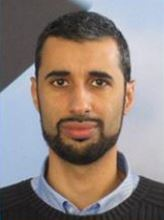
\includegraphics[width=1.5cm]{salim.jpg}
\end{wrapfigure}
% As a Data Scientist at Bull SAS, my expertise lies in developing robust data systems using Python OOP, Git, Docker, and MongoDB. My work has focused on multivariate time series processing and advanced machine learning techniques, utilizing tools such as scipy, sklearn, and tensorflow2/keras. I've been instrumental in High-Performance Computing (HPC) projects, optimizing workflows through Slurm and Optuna. My contributions include algorithm development in areas like image processing and recognition, driven by a commitment to continuous learning and collaborative problem-solving in a high-tech industry setting.

Data Scientist at Ryax Technologies, designing AI workflow orchestration for low-code platforms that deploy analytics and AI workflows across hybrid Cloud--HPC infrastructures. Current work spans multi-objective Kubernetes/Slurm scheduling, LLM-powered automation with agents and RAG pipelines, and transparent execution from Edge to Cloud to HPC. Five years at Bull built deep HPC expertise in recommendation systems, performance modeling, burst-buffer sizing, workflow optimization, production Python, multivariate time series, and scientific signal/image processing.

% As a Data Scientist, I have a solid background in Python OOP, classical Machine Learning tools, and some databases. My experience includes multivariate time series analysis and machine learning, utilizing tools like scipy, sklearn, and tensorflow2/keras. In my recent role at Bull SAS, I contributed to High-Performance Computing (HPC) projects, focusing on workflow optimization and HPC simulation, using tools such as Slurm and Optuna. My work also involves algorithm development in areas such as recognition and image processing. I am keen on continuous learning and collaboratively addressing new challenges.


% Accomplished Data Scientist with a keen interest in solving complex problems. Proficient in leveraging Python, Git, Docker, and MongoDB to create and manage efficient data systems. I have developed key skills in multivariate time series processing and machine learning, largely due to my consistent use of tools such as scipy, sklearn, and tensorflow2/keras. My background in scientific signal and image processing has provided a solid foundation for algorithm development involving recognition, alpha matting, classification, and segmentation. Recently, I have embarked on a journey to understand the nuances of High Performance Computing, using tools like slurm and nipype, and delving into data placement policies. As I continue to learn and grow in this field, I look forward to tackling new challenges and contributing to team successes.

% \blindtext[1]
